% Mercedes Roman Ruiz
\begin{table}[h]
    \centering
    \begin{tabular}{lr}
        \textbf{Cuenta de Resultados - 1ª Decisión} & \textbf{€} \\
        \hline
        \textbf{Ingresos por ventas}                & \textbf{1221875} \\
        Valor Stock inicial                         & 129336 \\
        Componentes comprados                       & 0 \\
        Adquisición de materias primas              & 510720 \\
        Funcionamiento máquinas                     & 72470 \\
        Salarios mecanizado                         & 182822 \\
        Salarios montaje                            & 119977 \\
        Control de calidad                          & 2839 \\
        Transporte                                  & 38100 \\
        Menos valor de stock final                  & 315017 \\
        \cline{2-2}
        \textbf{Coste de las ventas}                & 741247 \\
        \cline{2-2}
        \textbf{Beneficio Bruto}                    & 480628 \\
        Gastos generales                            & 499677 \\
        Seguros recibidos                           & 0 \\
        Amortización                                & 26770 \\
        \cline{2-2}
        \textbf{EBIT}                               & -45819 \\
        Ingresos financieros                        & 2250 \\
        \textbf{Gastos financieros}                 & \textbf{0} \\
        \cline{2-2}
        \textbf{Beneficio antes de impuestos}       & \textbf{-43569} \\
        Impuestos                                   & 0 \\
        \cline{2-2}
        \textbf{Resultado neto}                     & \textbf{-43569} \\
        \textbf{Beneficio por acción (cents)}       & \textbf{-1,09} \\
        \textbf{Pago de dividendos}                 & \textbf{0} \\
        \cline{2-2}
        Transferido a reservas                      & -43569 \\
        Reservas acumuladas                         & -186085 \\
        \cline{2-2}
        \textbf{Reservas totales}                   & \textbf{-229654}
    \end{tabular}
\end{table}

\begin{table}[h]
    \centering
    \begin{tabular}{|c|r|}
        \hline
        Margen Explotación  & -3,75 \% \\
        Margen Operativo    & -3,57 \% \\
        Margen Neto         & -3,57 \% \\
        ROA                 & -1,09 \% \\
        ROE                 & -1,16 \% \\
        Rotación            & 29,01 \% \\
        Endeudamiento       & 11,71 \% \\
        \hline
    \end{tabular}
\end{table}

\section*{Un Inicio Ambicioso: Activar la Demanda sin Asegurar la Capacidad}

La primera decisión supone el inicio de la gestión directa del equipo sobre IndusMoney y marca un punto de inflexión en la orientación estratégica de la compañía. A pesar de que el trimestre anterior había cerrado con beneficios, la empresa partía de una situación estructuralmente frágil, con reservas acumuladas negativas, lo que evidenciaba que los resultados positivos recientes no eran suficientes para garantizar la estabilidad a medio plazo.

En este contexto, la dirección opta por una estrategia claramente orientada a la activación de la demanda y al refuerzo del posicionamiento comercial. Se decide aumentar de forma significativa la inversión en publicidad corporativa y por producto en los tres mercados principales, con especial énfasis en el canal de Internet, complementando esta apuesta con una mejora del desarrollo web. Esta estrategia se apoya en una política de precios moderada, evitando competir agresivamente por precio y buscando transmitir una propuesta de valor sólida y coherente.

El objetivo de esta primera decisión no es maximizar el beneficio inmediato, sino sentar las bases para un crecimiento futuro sostenido, incrementando la visibilidad de la marca y estimulando la entrada de pedidos.

\section*{Estrategia Comercial Ambiciosa frente a una Política Operativa Conservadora}

Mientras la estrategia comercial adopta un enfoque expansivo, las decisiones operativas se mantienen deliberadamente prudentes. No se realizan ampliaciones de fábrica ni adquisiciones de nueva maquinaria, se conservan dos turnos de trabajo y se establece un nivel moderado de mantenimiento. Paralelamente, se refuerza ligeramente la plantilla mediante la contratación y formación de nuevos trabajadores, anticipando un crecimiento progresivo de la actividad sin incurrir en grandes inversiones estructurales.

Sin embargo, esta prudencia operativa no se traslada al área de aprovisionamiento. La política de compra de materias primas se apoya principalmente en adquisiciones spot y en un volumen reducido de aprovisionamiento a medio plazo. Esta decisión, orientada a limitar riesgos financieros y de almacenamiento, acaba convirtiéndose en un factor limitante cuando la demanda comienza a activarse como consecuencia de la inversión comercial.

El resultado es un claro desajuste entre la demanda generada y la capacidad real del sistema productivo para atenderla. Una parte significativa de los pedidos potenciales no puede ser satisfecha, lo que reduce de forma notable la efectividad de la estrategia comercial y limita el crecimiento de las ventas reales.

\section*{Resultados Económicos: Margen Bruto Positivo, Resultado Final Negativo}

Este desajuste entre áreas se refleja de manera directa en la cuenta de resultados. A pesar de que el beneficio bruto alcanza los 480.628 €, evidenciando que la actividad productiva genera margen a nivel operativo básico, este resultado es insuficiente para absorber el conjunto de gastos generales y costes estructurales asociados a una empresa en plena actividad.

La evolución de los distintos niveles de resultado muestra con claridad este fenómeno:

\begin{figure}[h]
  \centering
  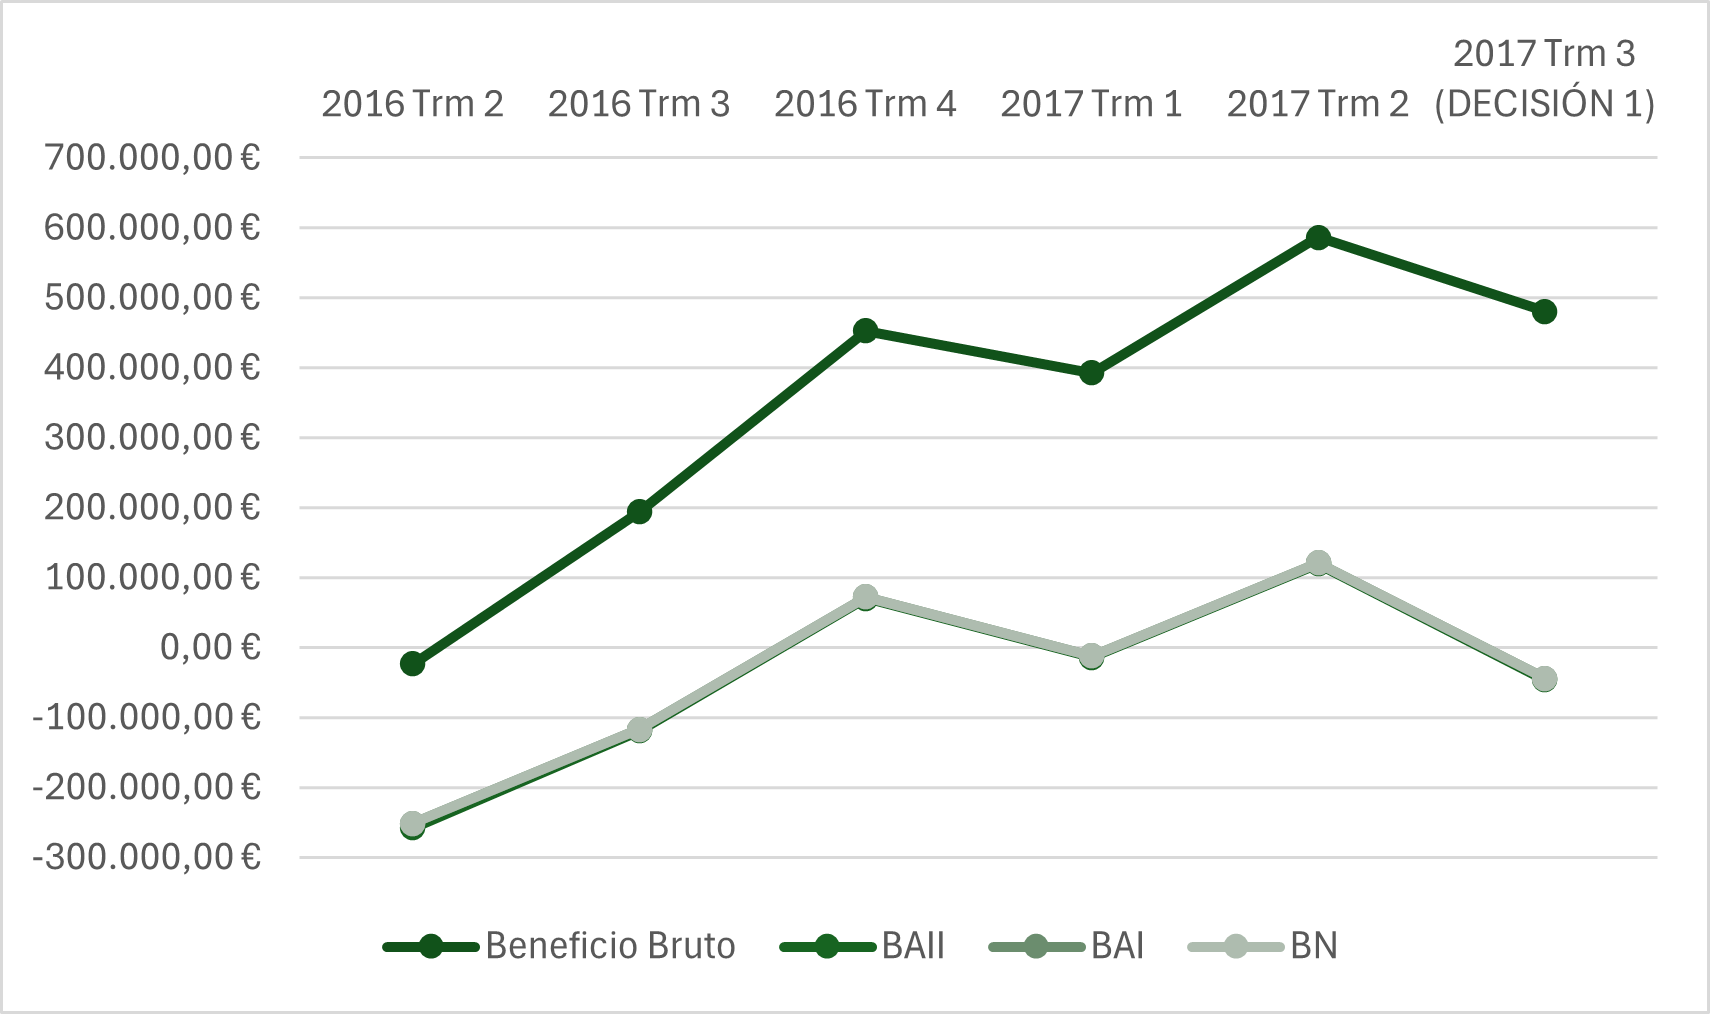
\includegraphics[width=\columnwidth]{Imagenes/decision1_beneficiobruto.png}
\end{figure}

El resultado de explotación (BAII) se sitúa en valores negativos (-45.819 €), confirmando que la estructura de costes fijos y operativos supera la capacidad de generación de ingresos del trimestre. Como consecuencia, el resultado antes de impuestos y el resultado neto también entran en terreno negativo, cerrando el periodo con unas pérdidas de 43.569 €.

Estas pérdidas provocan un nuevo deterioro de las reservas acumuladas, reforzando la idea de que el crecimiento comercial, cuando no va acompañado de una capacidad operativa alineada, puede convertirse en un factor de erosión del valor económico.

\section*{Deterioro de la Eficiencia: Márgenes en Terreno Negativo}

El análisis de los márgenes permite profundizar en la pérdida de eficiencia experimentada durante el trimestre. Tanto el margen de explotación como el margen operativo y el margen neto entran en valores negativos, indicando que la empresa pierde dinero por cada euro vendido.

\begin{figure}[h]
  \centering
  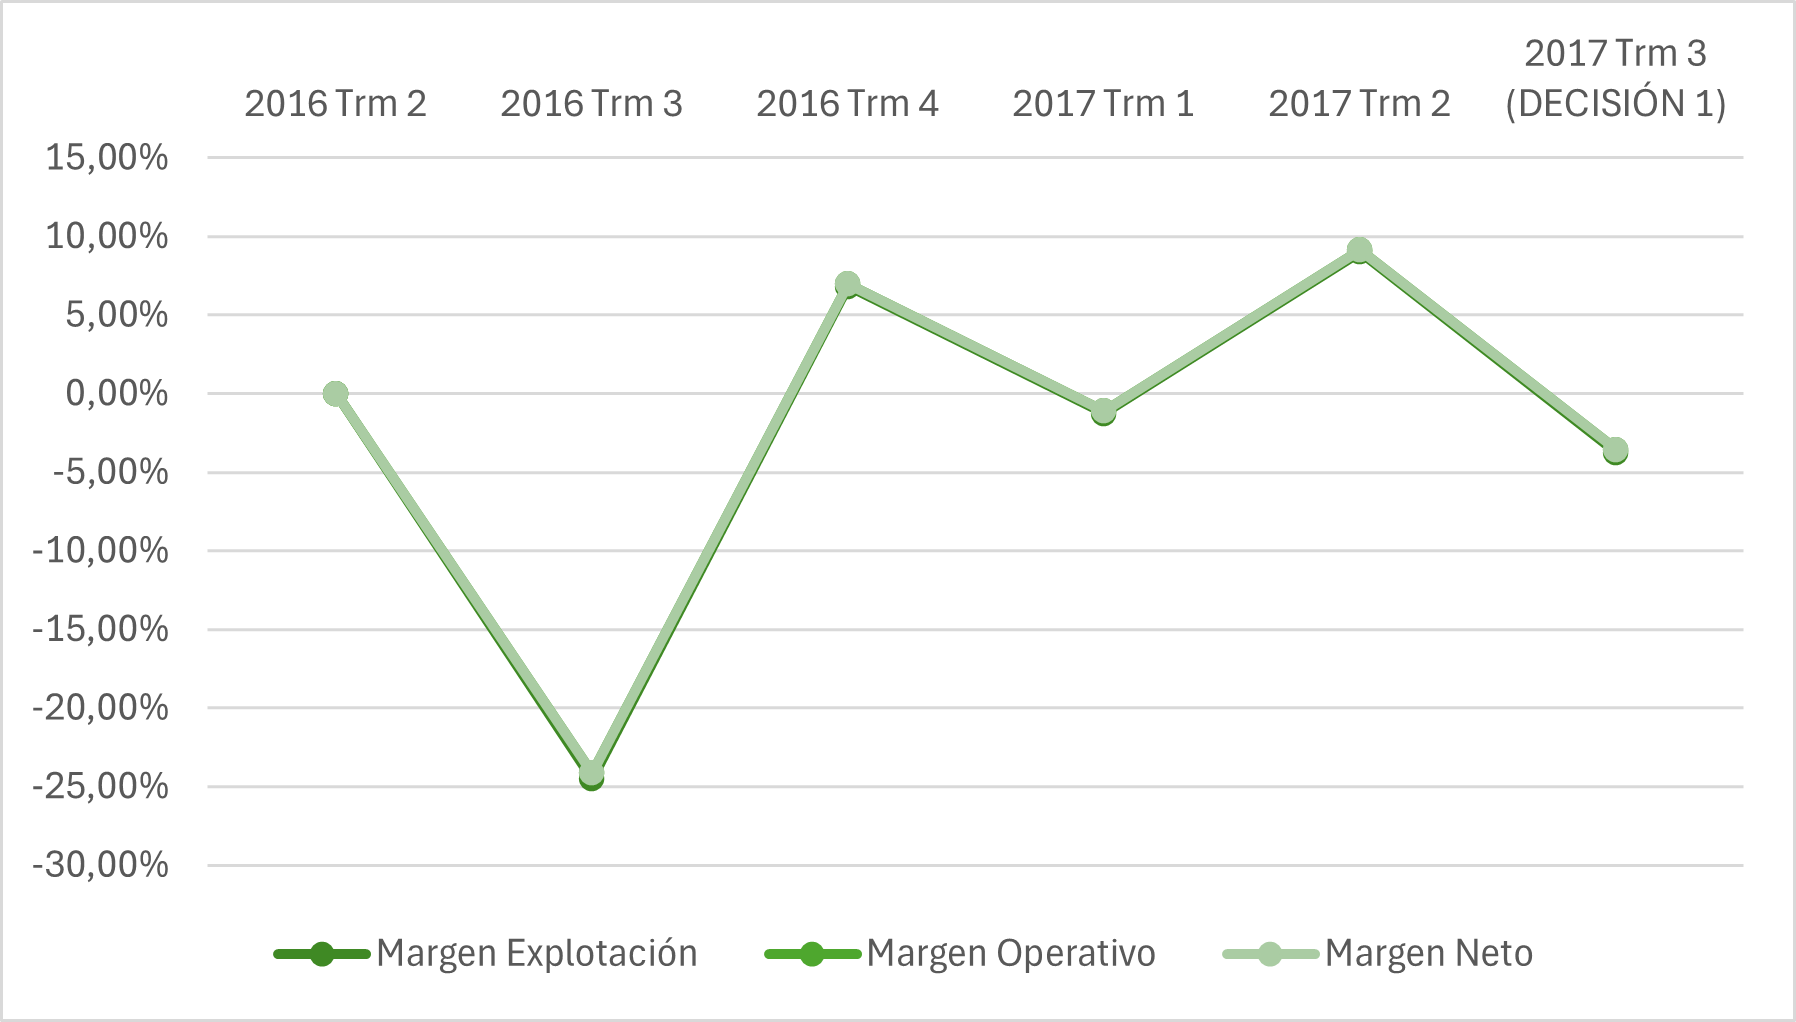
\includegraphics[width=\columnwidth]{Imagenes/decision1_margenes.png}
\end{figure}

Este comportamiento confirma que el problema no reside en la ausencia de actividad, sino en una estructura de costes sobredimensionada para el nivel real de ventas alcanzado. Los costes asociados al funcionamiento de la empresa —salarios, mantenimiento, gastos generales— se ejecutan con normalidad, mientras que los ingresos no crecen al ritmo esperado debido a las limitaciones en el suministro y la producción.

La empresa entra así en una fase en la que el crecimiento comercial no se traduce en rentabilidad, anticipando la necesidad de revisar la coordinación entre las decisiones comerciales y operativas en los siguientes trimestres.

\section*{Más Actividad sin Apalancamiento: Un Crecimiento Mal Capturado}

A pesar de los malos resultados económicos, algunos indicadores muestran señales de aumento de la actividad. La rotación de activos experimenta una mejora significativa, lo que indica un uso más intensivo de los recursos disponibles y un mayor dinamismo comercial.

\begin{figure}[h]
  \centering
  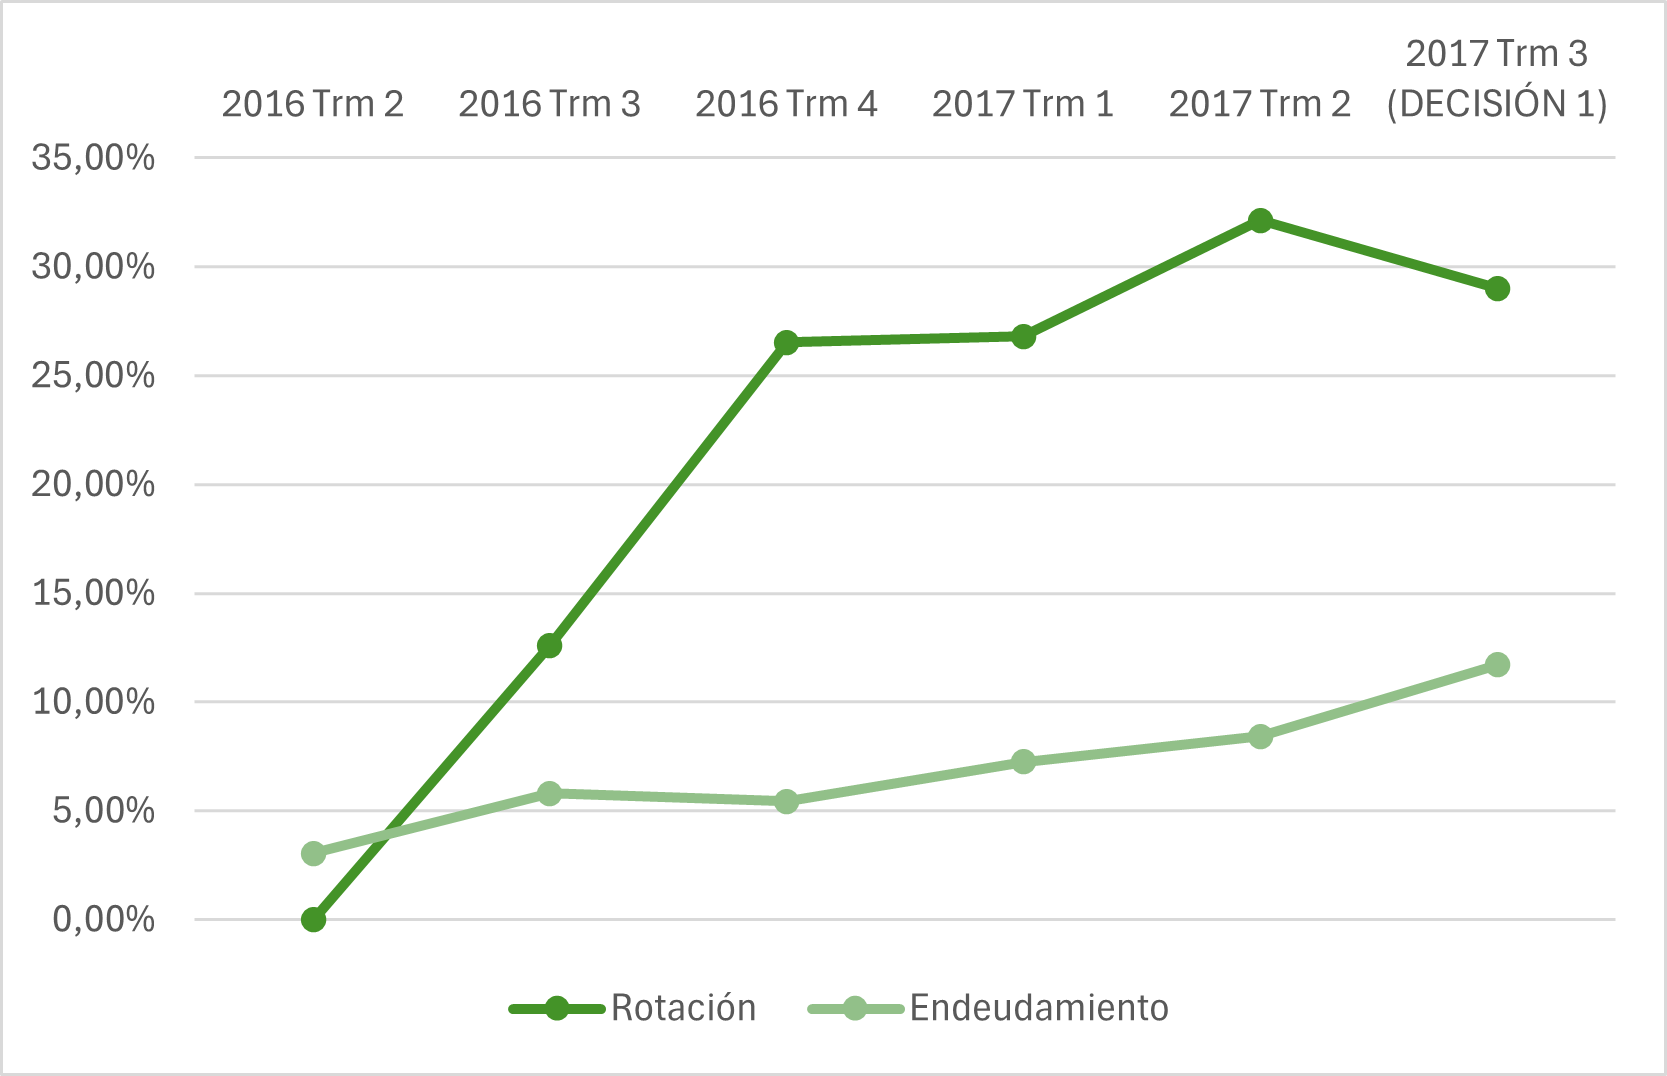
\includegraphics[width=\columnwidth]{Imagenes/decision1_endeudamiento.png}
\end{figure}

Este incremento de la actividad se produce sin recurrir a un aumento relevante del endeudamiento. La empresa mantiene una política financiera conservadora, evitando la financiación externa y sosteniendo su crecimiento mediante recursos propios y pasivo corriente. Esta ausencia de apalancamiento confirma que el problema del trimestre no es financiero, sino operativo.

No obstante, la mejora en la rotación no se traduce en creación de valor, ya que la empresa no consigue capturar rentabilidad a partir del mayor volumen de actividad.

\section*{Rentabilidad Negativa: Impacto Directo sobre el Accionista}

El deterioro de la eficiencia operativa se traslada directamente a los indicadores de rentabilidad. Tanto la rentabilidad económica (ROA) como la rentabilidad financiera (ROE) presentan valores negativos, evidenciando que ni los activos ni los fondos propios están generando retornos positivos en este periodo.

\begin{figure}[h]
  \centering
  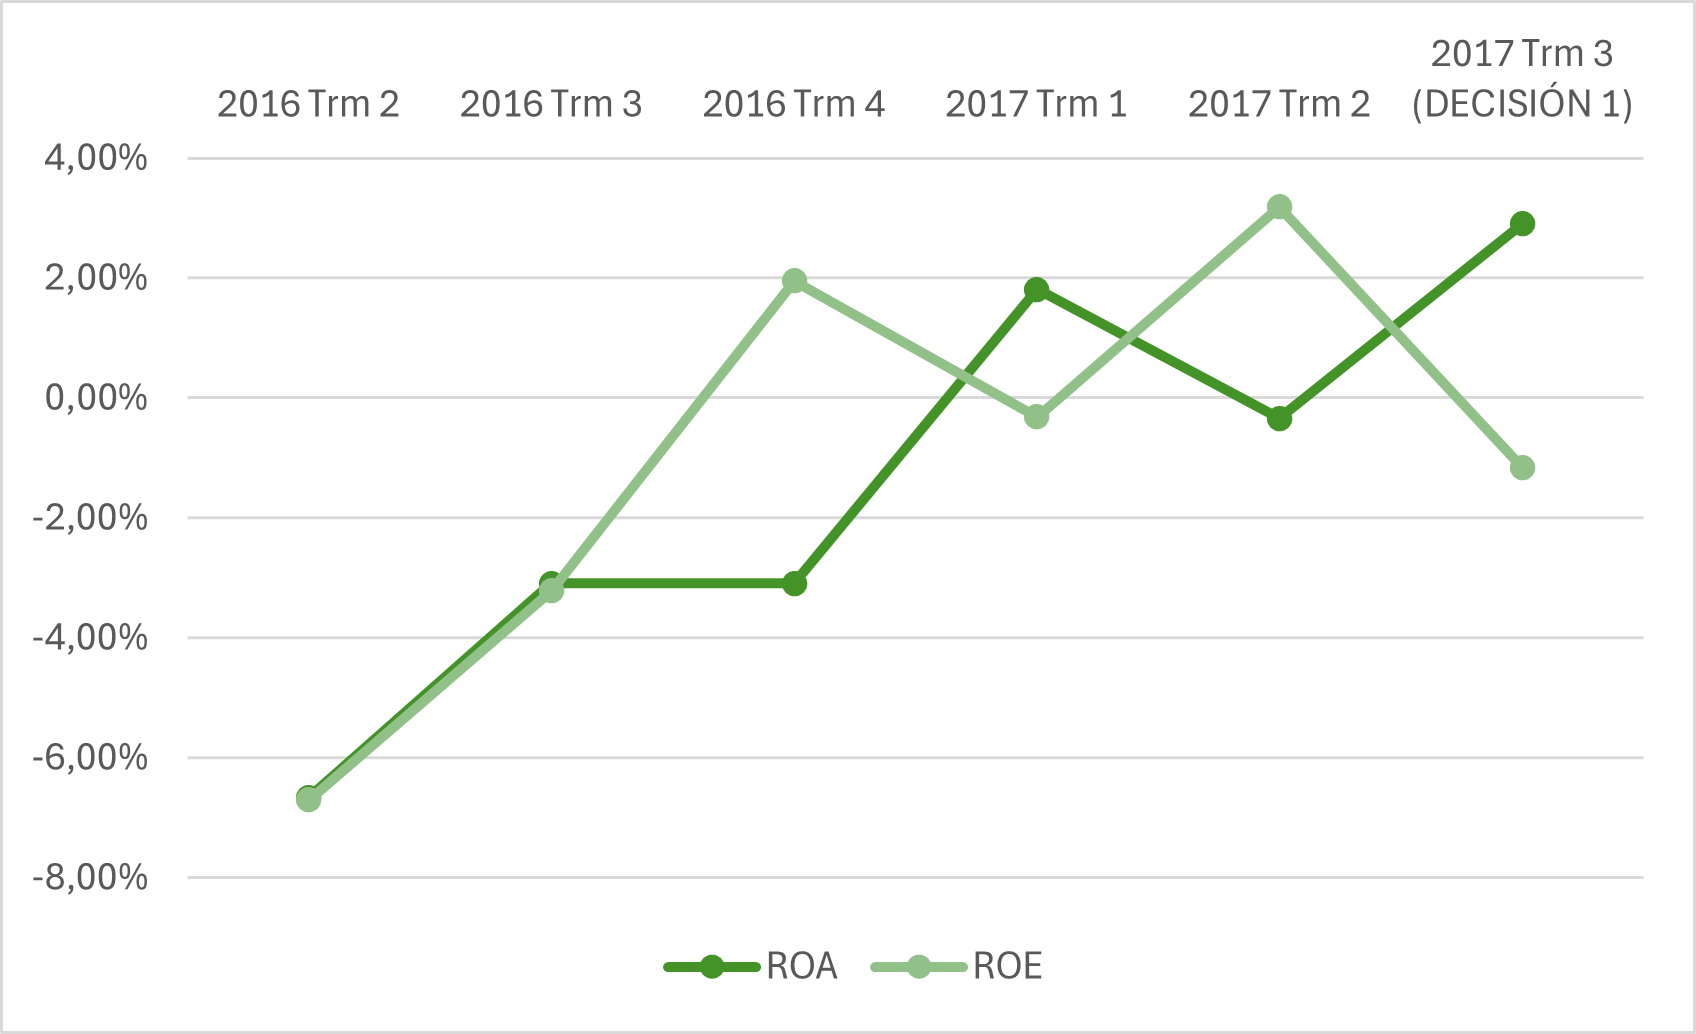
\includegraphics[width=\columnwidth]{Imagenes/decision1_ROAROE.png}
\end{figure}

Este resultado es especialmente relevante al producirse en ausencia de endeudamiento financiero significativo. La rentabilidad negativa no es consecuencia de un exceso de apalancamiento, sino del uso ineficiente de los recursos disponibles. La empresa destruye valor para el accionista desde la propia operativa, lo que convierte esta decisión en un primer aviso estratégico dentro de la simulación.

\section*{Primer Aviso Estratégico: Un Problema de Sincronización}

La primera decisión deja una conclusión clara y coherente con los resultados obtenidos. La estrategia adoptada es razonable en su planteamiento, al buscar activar la demanda y reforzar la posición de mercado de la empresa, pero resulta deficiente en su ejecución temporal. La falta de sincronización entre la política comercial y la capacidad operativa impide transformar el esfuerzo realizado en resultados económicos positivos.

Este trimestre no representa un colapso financiero, pero sí un aviso temprano. El crecimiento sin una base operativa alineada genera pérdidas, erosiona el patrimonio y anticipa riesgos mayores si no se corrigen estos desajustes. Las decisiones futuras deberán centrarse en ajustar el aprovisionamiento, mejorar la eficiencia operativa y convertir la actividad generada en rentabilidad sostenible.


\begin{table}[h]
    \centering
    \begin{tabular}{lr}
        \textbf{Balance - 1ª Decisión}               & \textbf{€} \\
        \hline
        \textbf{Activo fijo}                & \\
        Terreno                             & 50000 \\
        Bienes inmuebles                    & 250000 \\
        Valor de las máquinas               & 1044100 \\
        \cline{2-2}
        \textbf{Total activo fijo}          & \textbf{1344100} \\
        \textbf{Activo Circulante}          & \\
        Inventario - Productos              & 51723 \\
        Inventario - Componentes            & 0 \\
        Inventario - Materia Prima          & 263294 \\
        Deudores                            & 723625 \\
        Efectivo e Inversores               & 1829205 \\
        \cline{2-2}
        \textbf{Total activo circulante}    & \textbf{2867847} \\
        \cline{2-2}
        \textbf{Activo Total}               & \textbf{4211947} \\
        \textbf{Pasivo:}                    & \\
        Impuestos a pagar                   & 0 \\
        Acreedores                          & 441601 \\
        Línea de crédito / Descubierto      & 0 \\
        \cline{2-2}
        \textbf{Pasivo exigible}            & \textbf{441601} \\
        \textbf{Préstamos}                  & \textbf{0} \\
        \textbf{Activo neto}                & \textbf{3770346} \\
        \textbf{Fondos propios}             & \\
        Capital social                      & 4000000 \\
        Prima de emisión                    & 0 \\
        Reservas                            & -229654 \\
        \cline{2-2}
        \textbf{Patrimonio neto}            & 3770346 
    \end{tabular}
\end{table}

\begin{table}[h]
    \centering
    \begin{tabular}{|c|r|}
        \hline
        NOF & 2.426.246,00 € \\
        FM & -1.344.100,00 € \\
        EC & -3.770.346,00 € \\
        \hline
    \end{tabular}
\end{table}
